% id: 0192
% book: 쎈 중3-2 수학 · 02 삼각비의 활용
% section: 유형 04 일반 삼각형의 변의 길이; 두 변의 길이와 그 끼인각의 크기를 알 때
% figure: tikz:fig-0192
% answer: ⑤
% answer_source: 답지
% variant_level: 0 (원본 전사)
% 이 파일은 build.mjs 가 items.json 에서 만든다. 고칠 때는 items.json 을 고친다.
\smash{\raisebox{3.5mm}{\dmkichul{쎈 중3-2 수학 0192번 · 39쪽}}}
\noindent\begin{minipage}[t]{0.58\linewidth}\vspace{0pt}\raggedright 오른쪽 그림의 $\triangle\pt{ABC}$에서 $\seg{AC}=10$, $\seg{BC}=12$이고 $\cos C=\dfrac{4}{5}$일 때, $\seg{AB}$의 길이는?\end{minipage}\hfill\begin{minipage}[t]{0.4\linewidth}\vspace{0pt}\centering \resizebox{\ifdim\width>\linewidth\linewidth\else\width\fi}{!}{% 0192(본책 39쪽) — △ABC(AC=10, BC=12). 스캔 삽화를 TikZ 로 다시 그림. 답(AB)은 적지 않는다.
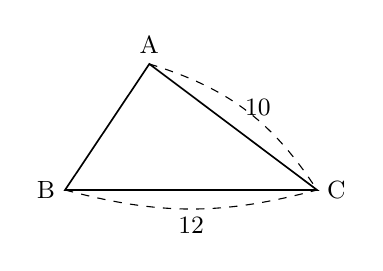
\begin{tikzpicture}[line width=0.6pt]
  \coordinate (B) at (0,0); \coordinate (C) at (3.2,0); \coordinate (A) at (1.07,1.6);
  \draw (A) -- (B) -- (C) -- cycle;
  \draw[dashed, line width=0.4pt] (A) to[bend left=20] (C);
  \draw[dashed, line width=0.4pt] (B) to[bend right=15] (C);
  \node[font=\small] at (2.45,1.05) {$10$};
  \node[font=\small] at (1.6,-0.45) {$12$};
  \node[font=\small, above] at (A) {A};
  \node[font=\small, left] at (B) {B};
  \node[font=\small, right] at (C) {C};
\end{tikzpicture}
}\end{minipage}\par
\begin{choices32}{\rule[-3ex]{0pt}{8ex}$\sqrt{13}$}{\rule[-3ex]{0pt}{8ex}$\sqrt{15}$}{\rule[-3ex]{0pt}{8ex}$\dfrac{3\sqrt{13}}{2}$}{\rule[-3ex]{0pt}{8ex}$\dfrac{3\sqrt{15}}{2}$}{\rule[-3ex]{0pt}{8ex}$2\sqrt{13}$}\end{choices32}
